% TEXINPUTS=.:$HOME/git/bvtex: latexmk  -pdf <main>.tex
\documentclass[xcolor=dvipsnames]{beamer}

\input{defaults}
\input{beamer/preamble}

\setbeamertemplate{navigation symbols}{}
% \setbeamertemplate{background}[grid][step=1cm]

\usepackage{siunitx}
\usepackage{xmpmulti}
\usepackage[export]{adjustbox}

\usepackage[outline]{contour}
\usepackage{tikz}
\usetikzlibrary{shapes.geometric, arrows}
\usetikzlibrary{positioning}

\definecolor{bvtitlecolor}{rgb}{0.98, 0.92, 0.84}
\definecolor{bvoutline}{rgb}{0.1, 0.1, 0.1}

\renewcommand{\bvtitleauthor}{Brett Viren}
\renewcommand{\bvtitle}{\LARGE 3D Field and Detector Response Calculations\\With Boundary Element Method}
\renewcommand{\bvtit}{LARF}
\renewcommand{\bvevent}{\Large DUNE FD Sim/Reco\\\today}
\renewcommand{\bvbeamerbackground}{}

\newcommand{\microboone}{MicroBooNE\xspace}


\begin{document}
\input{beamer/title.tex}
\input{beamer/toc.tex}

\section{Formalism}

\begin{frame}
  \frametitle{Detector Response}
  \begin{itemize}
  \item A single charge passing near a LArTPC wire \textbf{induces} a
    \textbf{current waveform} which is then \textbf{shaped and digitized}.
    \begin{itemize}\scriptsize
    \item Collection wires too, truly collected charge makes a short,
      current spike.
    \end{itemize}
  \item The waveform \textbf{of a single charge} depends, in fine
    detail, on the instantaneous values of the:
    \begin{itemize}\footnotesize
    \item \textbf{charge velocity} (vector), ie, drift velocity.
    \item \textbf{charge location} relative to the \textbf{wire of interest} as well
      as \textbf{every other electrode} in the vicinity.
    \end{itemize}
  \item In reality, we measure an \textbf{ensemble of superimposed
      waveforms} from multiple, \textbf{distributed charges}.
  \item We must \textbf{deconvolve} the ensemble waveforms
    with some \textbf{average response function} to produce a good
    measure of \textbf{distribution of drifting charge}.
  \end{itemize}
  
  \footnotesize
  $\rightarrow$ the more the average response function
  matches the the true, instantaneous response function the better
  the deconvolved LArTPC image.

\end{frame}


\begin{frame}
  \frametitle{Instantaneous Induced current}

  Current in $k^{th}$ wire due to charge $q$ at position $\vec{r}(t)$ at time $t$: \\
  \begin{center}
    $i_k(\vec{r}(t)) = q \times (\vec{E}_{weight,k} \cdot \vec{v})$      

    $\vec{v} = \mu \vec{E}_{drift}(\vec{r}(t))$ 
  \end{center}

  \begin{description}
  \item[Drift field] $\vec{E}_{drift}$ from applied high voltage
  \item[Weight field] $\vec{E}_{weight,k}$ constructed \textit{Shockley-Ramo} field.
  \item[Drift Velocity] $\vec{v}(t)$ determines (mean) drift path of an electron.
  \item[Mobility] $\mu = \mu(E_{drift})$ of the drifting charge in LAr.
  \end{description}

  \footnotesize
  ($\vec{E}_{weight,k}$ calculated by setting wire $k$ to 1V and all other electrodes to 0V.)

\end{frame}

\section{Calculating Detector Response}

\begin{frame}
  \frametitle{The Game}
  \begin{enumerate}
  \item Define electrode geometry (eg, some wires + cathode).
  \item Calculate scalar and vector fields:
    \begin{itemize}
    \item $\phi_{drift}$ and its $\vec{E}_{drift}$ for the given geometry.
    \item $\phi_{weight,k}$ and its $\vec{E}_{weight,k}$ for each wire of interest.
    \item $v$ velocity vector field.
    \item $i$ instantaneous scalar current field.
    \end{itemize}
  \item Step through vector vector field while sampling current field.
  \item Explore ways to average sampled currents to form \\
    \textbf{average response functions}.
  \end{enumerate}
\end{frame}

\begin{frame}
  \frametitle{The Boundary Element Method (BEM)}

  \begin{enumerate}
  \item Discretize electrode surfaces with a triangular mesh.
  \item Define potential boundary conditions on mesh elements.
  \item Integrate Laplace equation $\nabla^2\phi=0$.
  \item Fit integral equation to boundary values.
  \item Evaluate at points in the volume to get $\phi(\vec{r})$.
  \end{enumerate}

  A lot of math and code: rely on \href{http://gmsh.info/}{GMSH} for
  meshing (1-2) and \href{http://www.bempp.org/}{BEM++} for
  solving/evaluating (3-5).

\end{frame}

\begin{frame}
  \frametitle{Element Methods: Boundary vs. Finite}
  \begin{columns}
    \begin{column}{0.5\textwidth}
      BEM
      \begin{itemize}
      \item Meshes the surfaces.
      \item Fast for low surface-to-volume.\\($\vec{E}_{weight,k}$)
      \item Performance relies on relatively new math discoveries.
      \item Relatively few software implementations.
      \end{itemize}      
      \textbf{This work.}
    \end{column}
    \begin{column}{0.5\textwidth}
      FEM
      \begin{itemize}
      \item Meshes the volume.
      \item Fast for high surface-to-volume.\\($\vec{E}_{field}$)
      \item Adaptive meshes can improve performance.
      \item Many implementations, heavily used in industry.
      \end{itemize}      
      \textbf{Past 2D and new 3D $\rightarrow$}
    \end{column}
  \end{columns}
\end{frame}
\begin{frame}
  \frametitle{Plug for Leon Rochester's FEM Work}
  \begin{columns}
    \begin{column}{0.5\textwidth}
      \begin{center}
        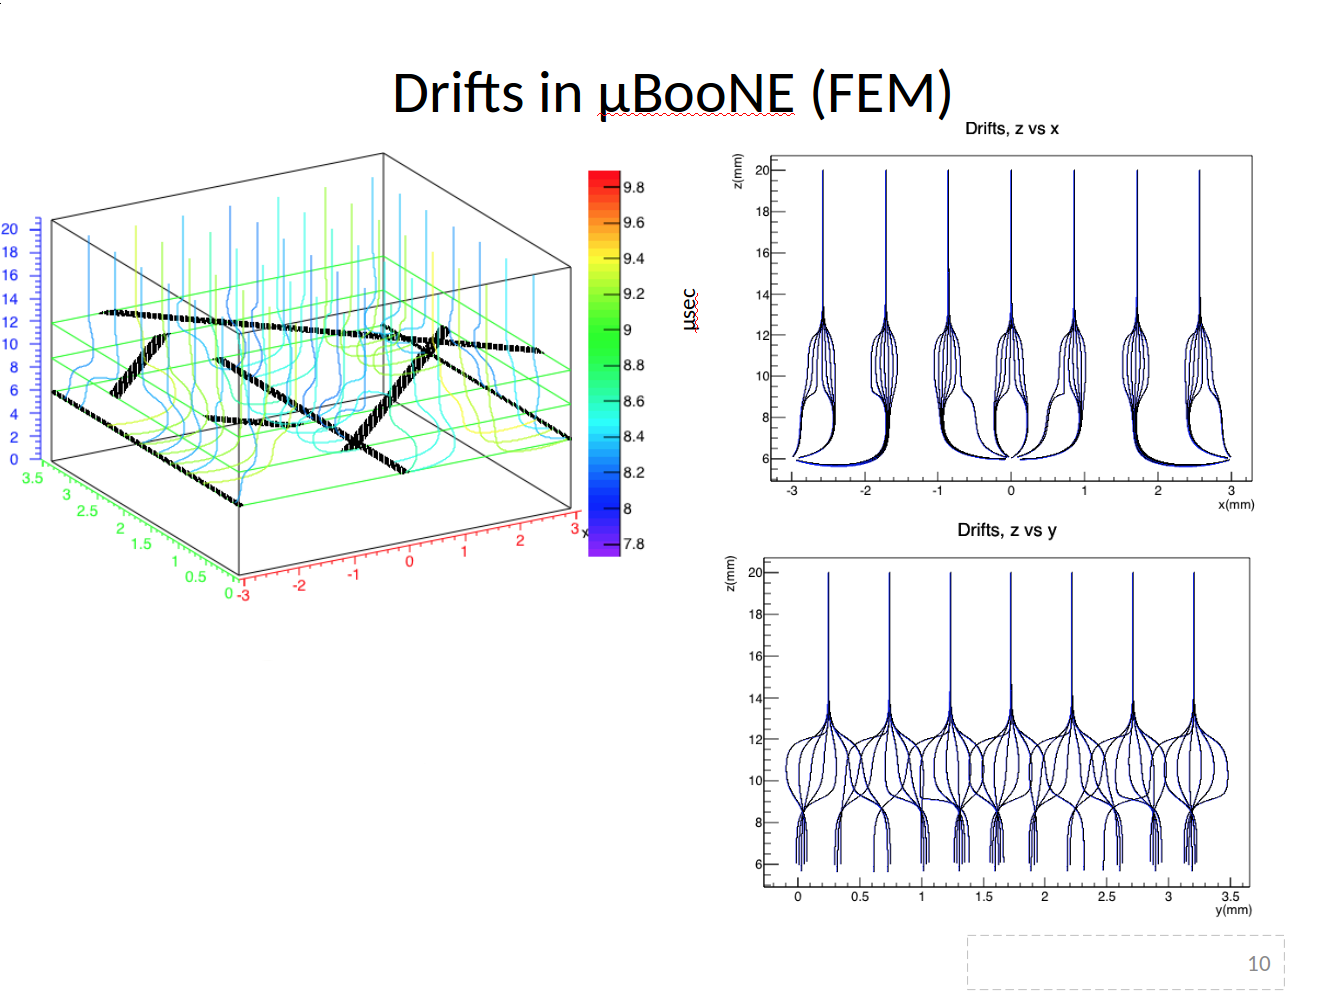
\includegraphics[width=\textwidth]{leon-drifts.png}
      \end{center}
    \end{column}
    \begin{column}{0.5\textwidth}
      \begin{center}
        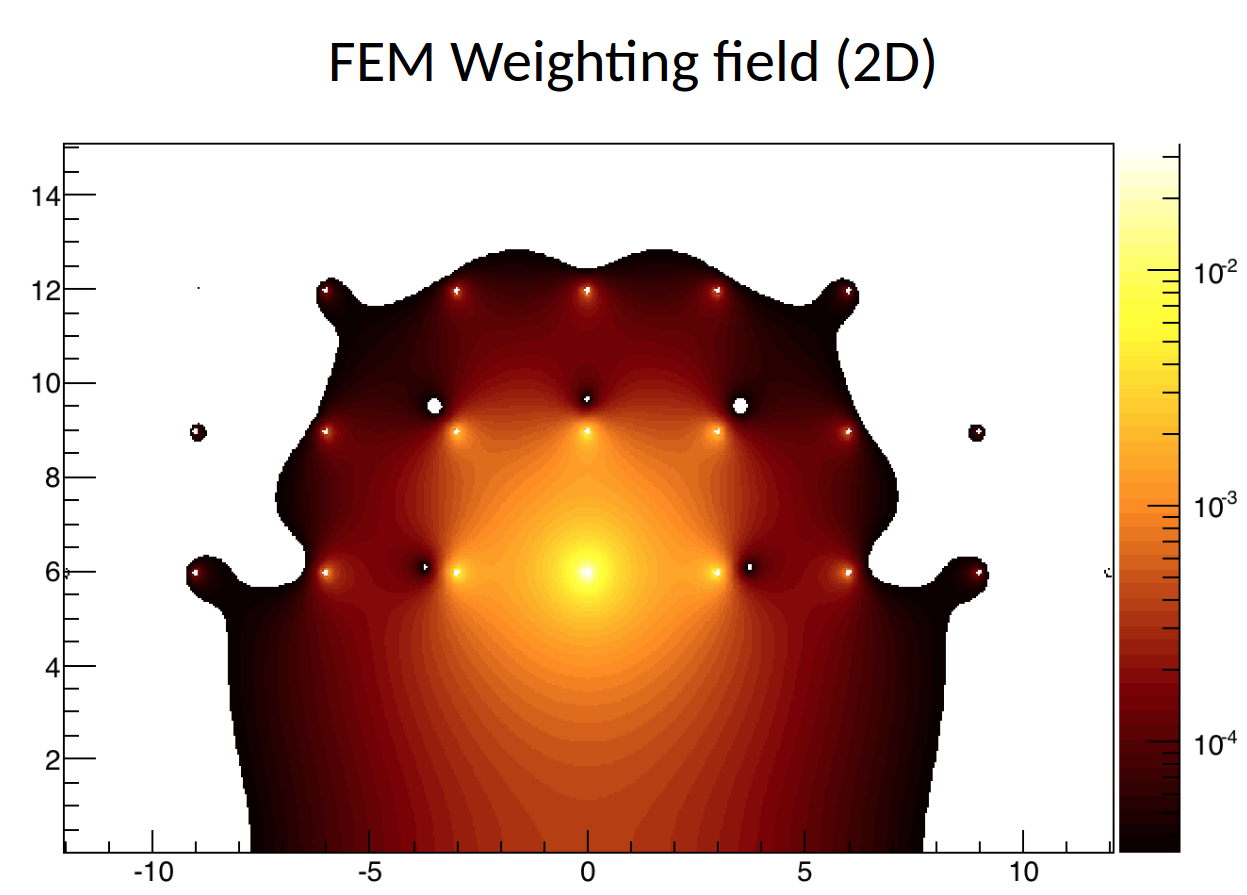
\includegraphics[width=\textwidth]{leon-weighting.png}        
      \end{center}
    \end{column}
  \end{columns}
  \begin{itemize}\footnotesize
  \item Contemporaneous and collaborative work with Leon Rochester @ SLAC.
  \item Custom C++/ROOT FEM code inspired by ICARUS' FORTRAN codes.
  \item Realizes the benefit of the FEM approach (eg, near-surface precision).
  \end{itemize}
  $\rightarrow$ Potential BEM/FEM hybrid to get the best of both.
\end{frame}

\section{Geometry}

\begin{frame}{Wires Meshes}

  \footnotesize

  \begin{columns}
    \begin{column}{0.3\textwidth}
      \begin{center}
        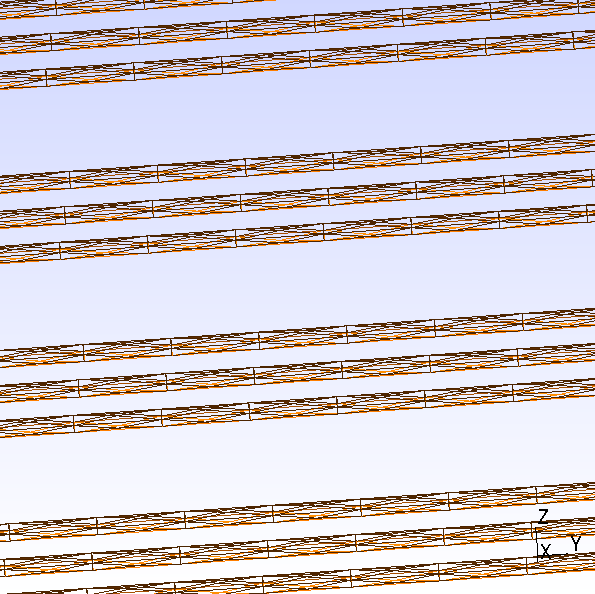
\includegraphics[height=0.4\textheight]{parallel-mesh.png}      
        
        ``Parallel'':\\3mm pitch and gap\\all wires parallel
      \end{center}
    \end{column}
    \begin{column}{0.3\textwidth}
      \begin{center}
        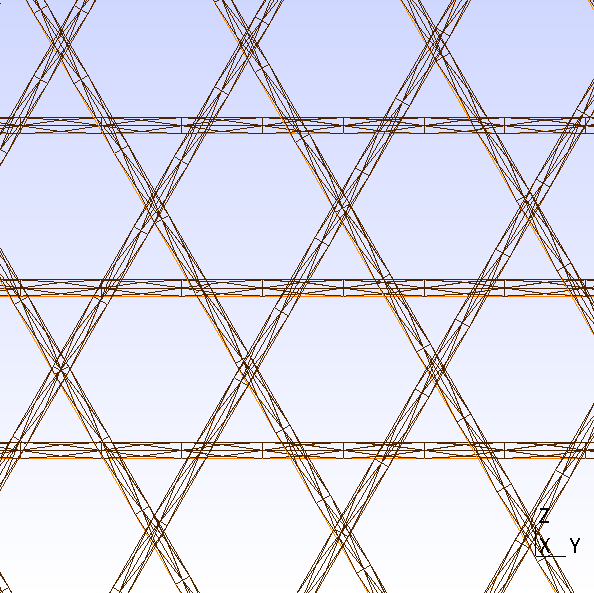
\includegraphics[height=0.4\textheight]{uboone-mesh.png}      

        ``\microboone''-like:\\3mm pitch and gap\\$60^\circ$ angles for U/V.
      \end{center}
    \end{column}
    \begin{column}{0.3\textwidth}
      \begin{center}
        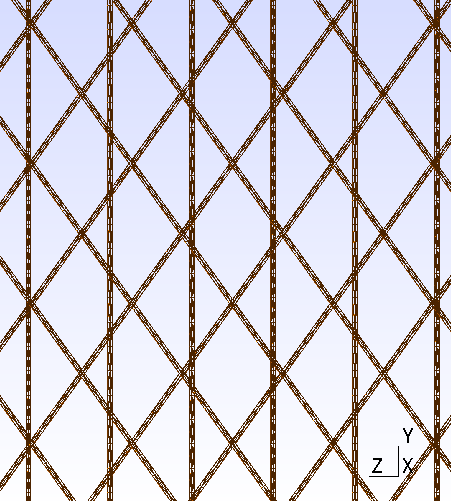
\includegraphics[height=0.4\textheight]{dune-mesh.png}      

        ``DUNE''-like:\\5mm pitch and gap\\$35.7^\circ$ angles for U/V.
      \end{center}
    \end{column}
  \end{columns}

  \vfill

  Wire generation is parameterized so easy to explore different wire patterns.
\end{frame}

\subsection{Parallel Wires / fake-2D}


\begin{frame}
  \frametitle{Parallel Wires - Slice Through Weighting Potentials}
  \begin{columns}
    \begin{column}{0.3\textwidth}
      \begin{center}
        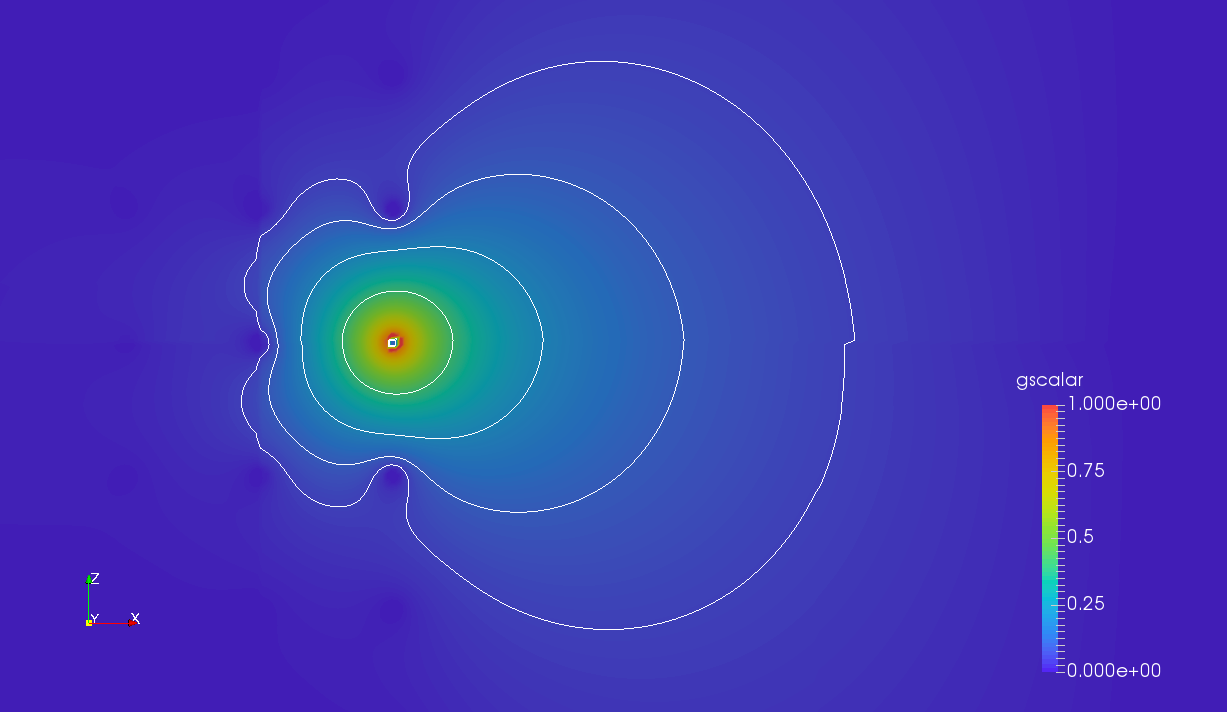
\includegraphics[height=2cm]{twodee-fine-u7.png}

        \scriptsize U plane
      \end{center}
    \end{column}
    \begin{column}{0.3\textwidth}
      \begin{center}
        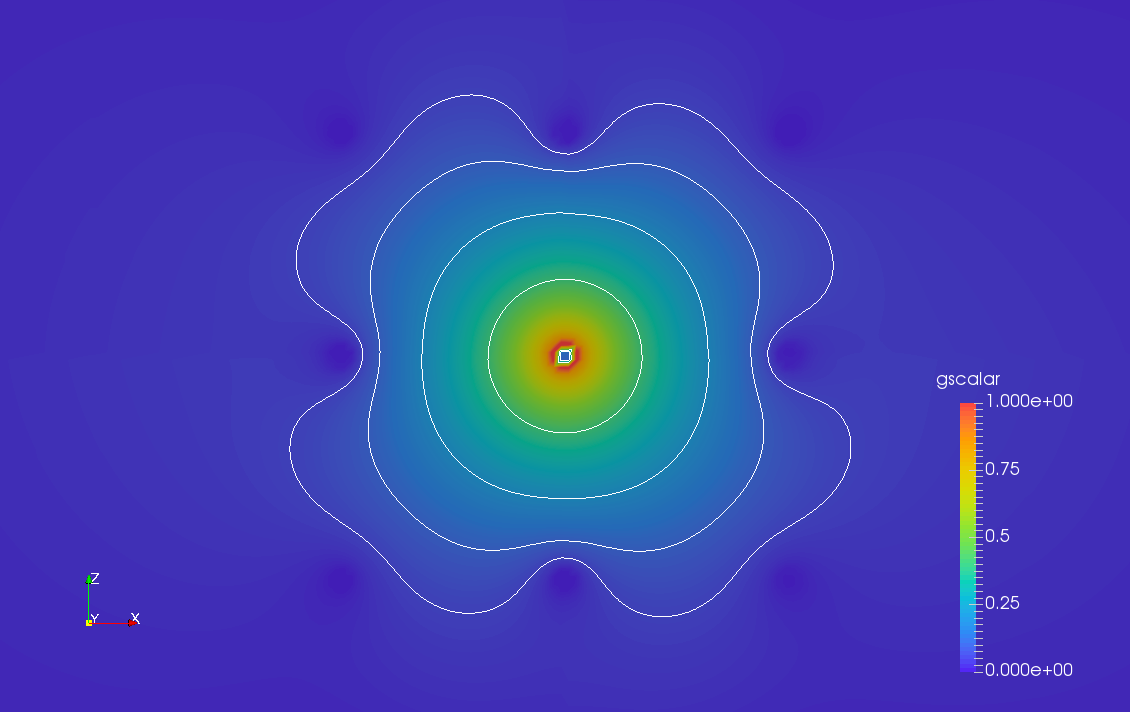
\includegraphics[height=2cm]{twodee-fine-v7.png}
        
        \scriptsize V plane
      \end{center}
    \end{column}
    \begin{column}{0.3\textwidth}
      \begin{center}
        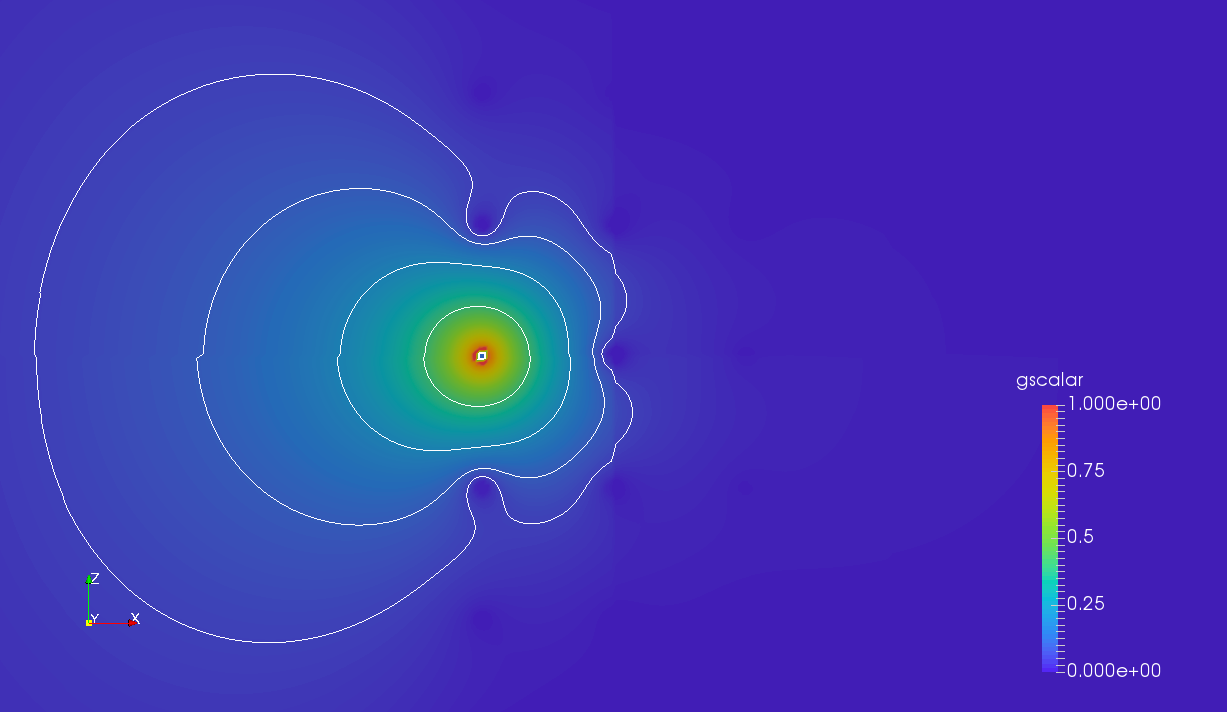
\includegraphics[height=2cm]{twodee-fine-w7.png}

        \scriptsize W plane
      \end{center}
    \end{column}
  \end{columns}

  \begin{itemize}\footnotesize
  \item X-Z slice through plane of symmetry (Y=0).
  \item Color shows weighting potential: 0-100\%.
  \item Lines: 5\%, 10\%, 20\%, 40\% weights.
  \end{itemize}

\end{frame}


\begin{frame}
  \frametitle{Weighting Potential - 2D vs ``2D''}

  \vspace{-5mm}

  \begin{columns}
    \begin{column}{0.5\textwidth}
      \begin{center}
        \includegraphics[height=0.65\textheight,page=5,angle=-90,clip,trim=0 0 0 5mm]{GarfieldSimulation-BoYu.pdf}

        \scriptsize Garfield 2D calculation from Bo
      \end{center}
    \end{column}
    \begin{column}{0.5\textwidth}
      \begin{center}
        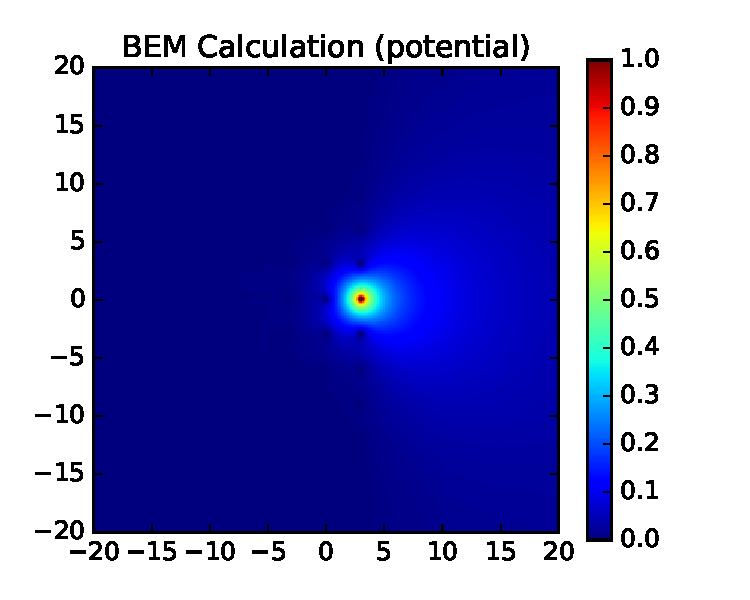
\includegraphics[height=0.65\textheight]{parallel-near-d11.pdf}

        \scriptsize 3D BEM, parallel wires, sliced at Y=0.
      \end{center}
    \end{column}
  \end{columns}

  \begin{center}\footnotesize
    Initial, qualitative agreement.  

    More checks would be good but, good enough to continue.
  \end{center}

\end{frame}


\subsection{MicroBooNE-like}

\begin{frame}
  \frametitle{Wire Geometry with Cathode Plane}
  \begin{columns}
    \begin{column}{0.5\textwidth}
      \begin{center}
        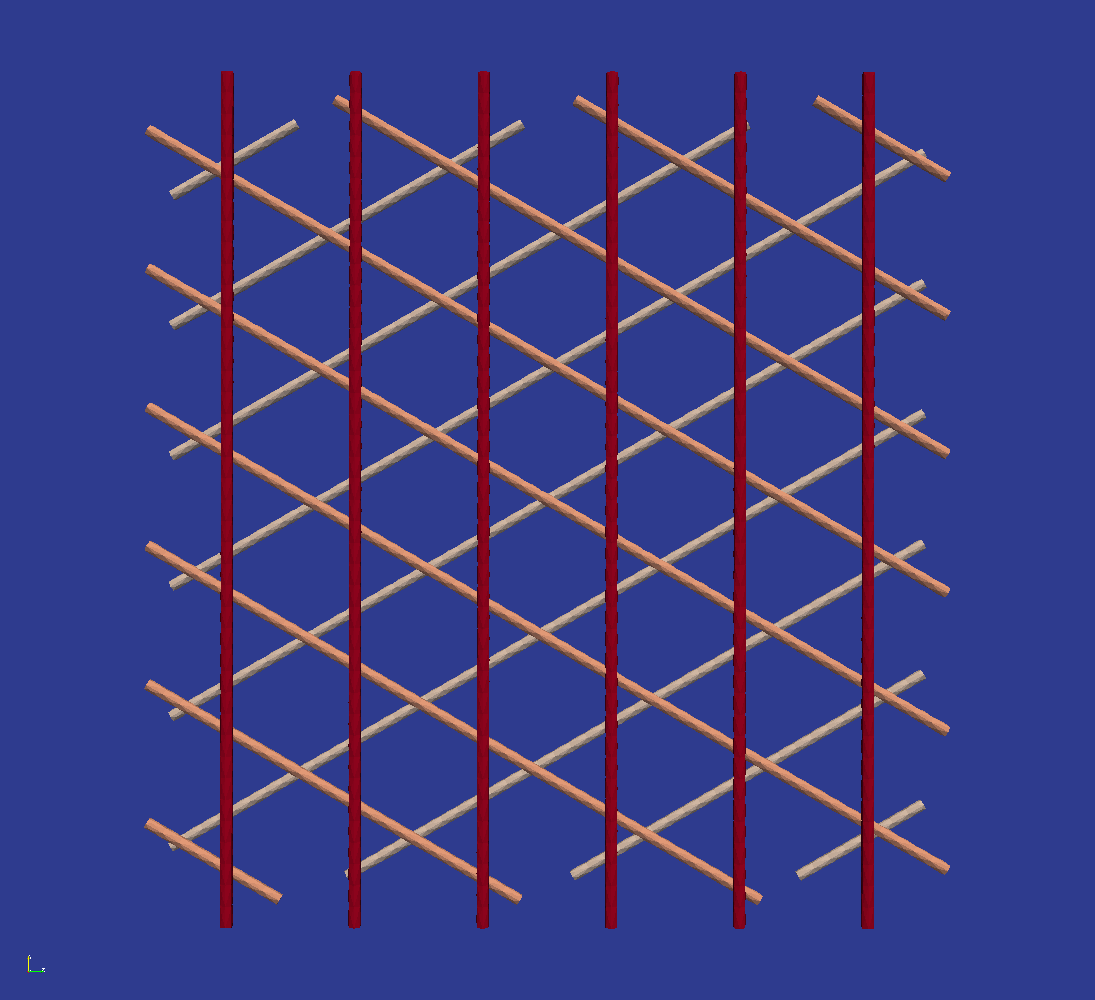
\includegraphics[width=\textwidth]{wires-flat.png}
      \end{center}
    \end{column}
    \begin{column}{0.5\textwidth}
      \begin{center}
        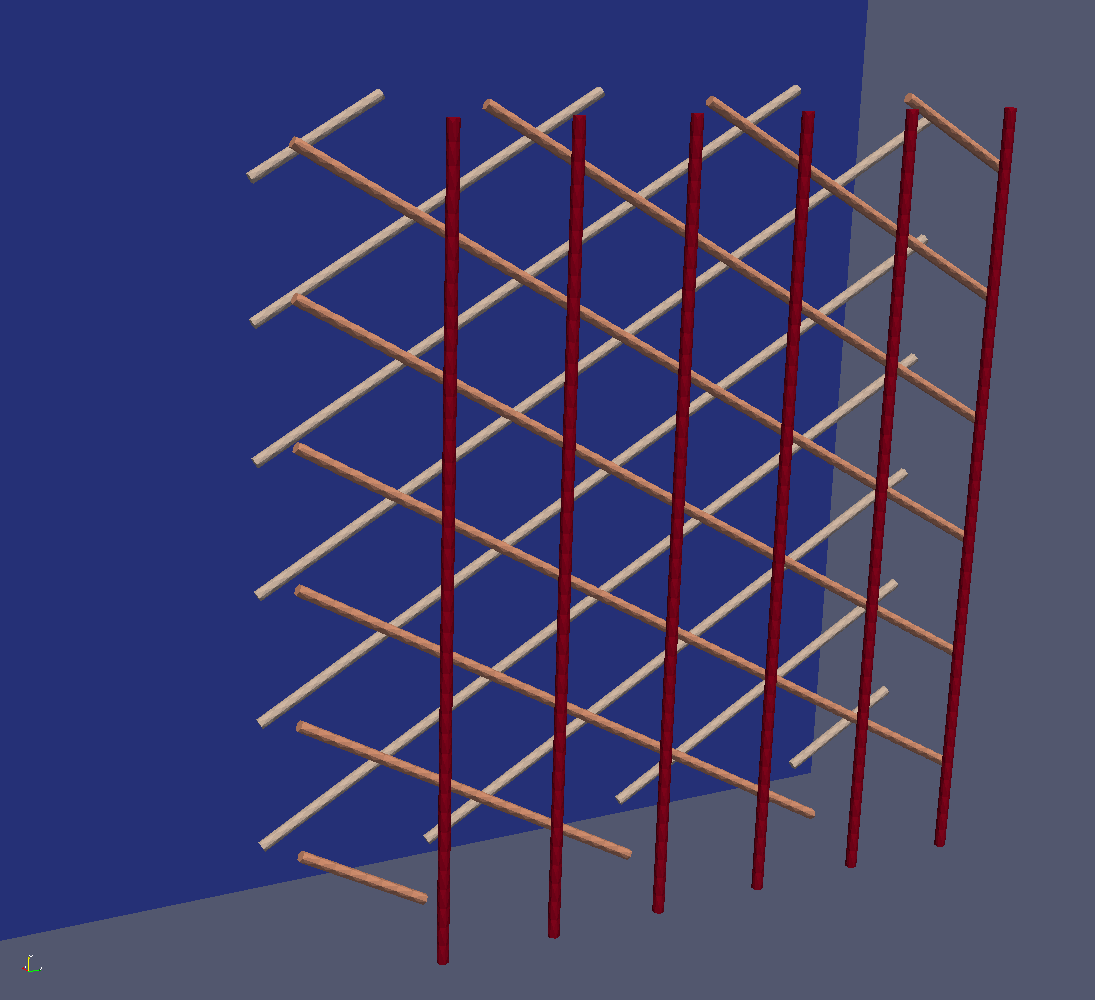
\includegraphics[width=\textwidth]{wires-iso.png}
      \end{center}
    \end{column}
  \end{columns}
  
  \begin{center}
    Wires parameterized by pitch, angle, bounding box, radius.
  \end{center}
\end{frame}

\begin{frame}
  \frametitle{V-plane $\vec{E}_{weight}$ Slices}
  \begin{center}
      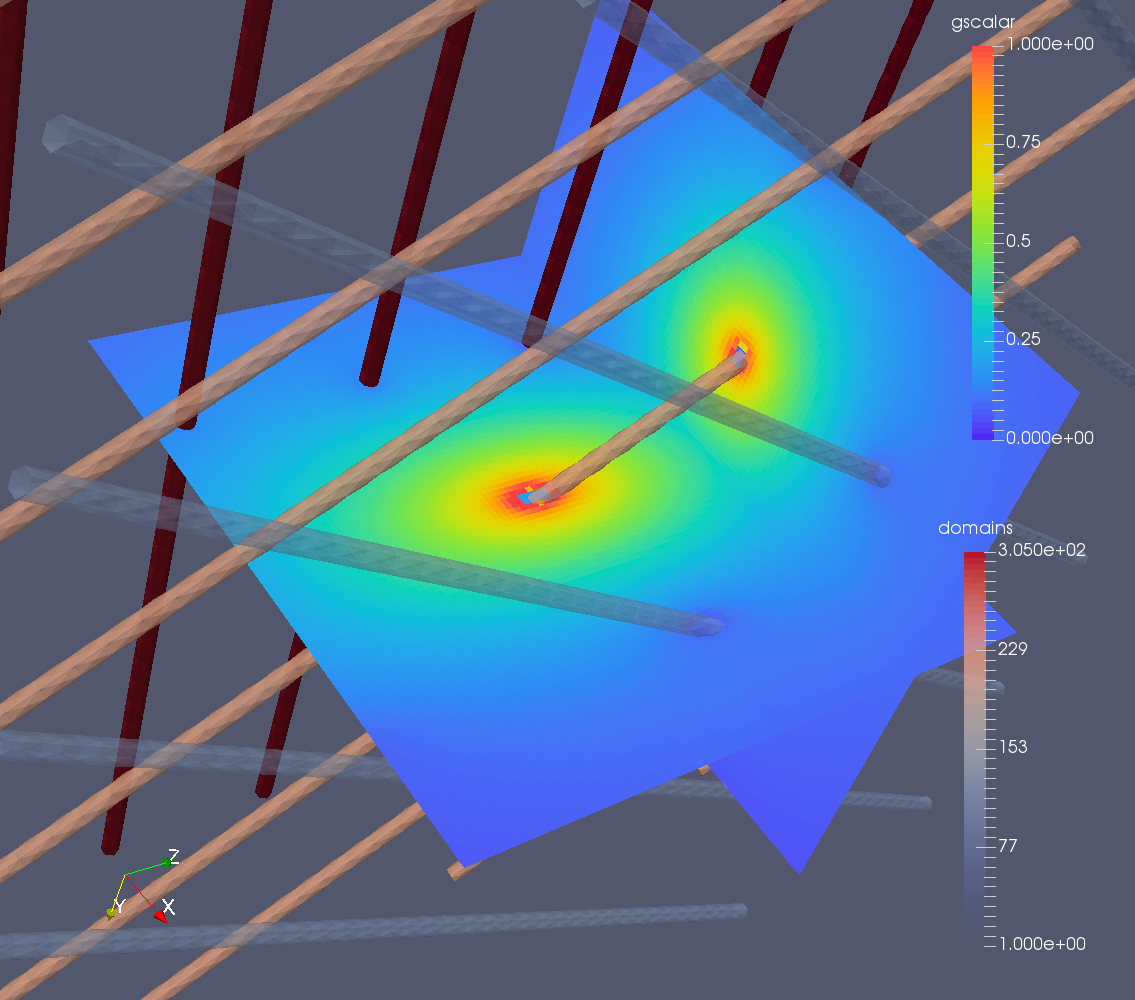
\includegraphics[width=0.7\textwidth]{cap-vweight-field-fine-slices.png}
  \end{center}
\end{frame}

\begin{frame}
  \frametitle{Paraview stepping from line source}
  \begin{center}
      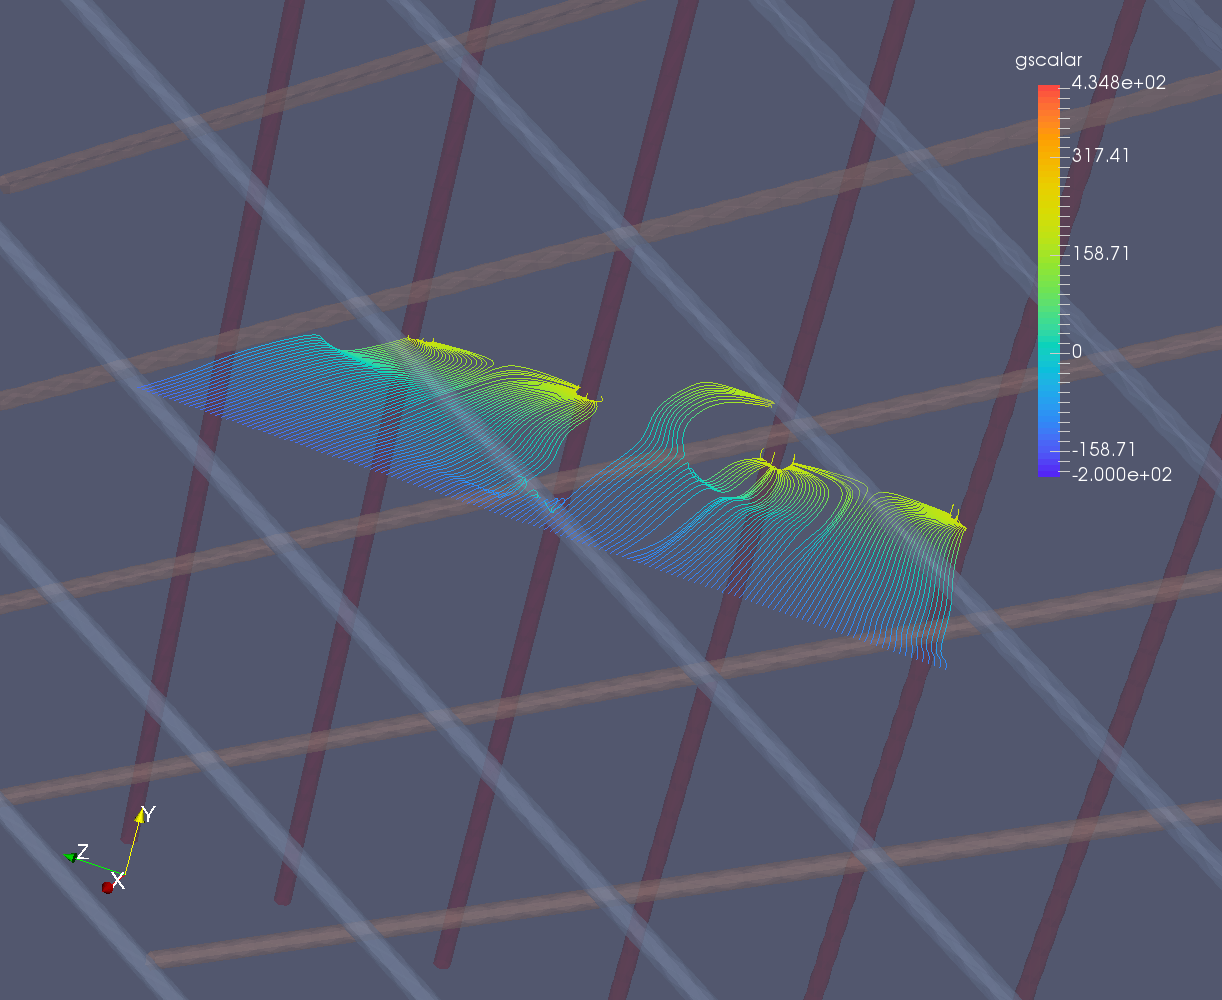
\includegraphics[width=0.7\textwidth]{track-drift-2.png}
  \end{center}
\end{frame}

\section{Initial Response Function Results}

\begin{frame}
  \frametitle{Initial Response Function Results}
  \begin{columns}
    \begin{column}{0.7\textwidth}
      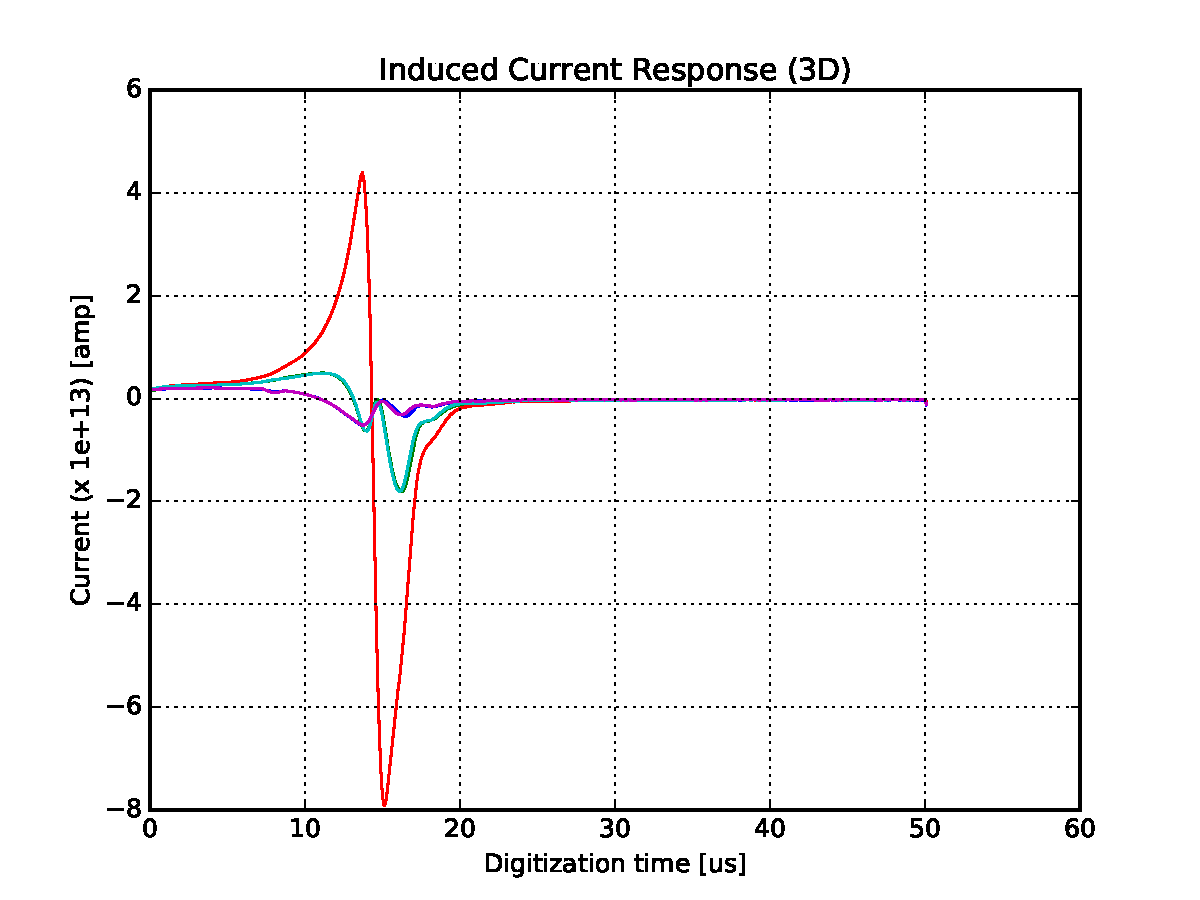
\includegraphics[width=\textwidth]{qad-response.pdf}

      \footnotesize
      Response for charge near a U-plane wire and charge passing near
      its nearest and next-nearest wires.

    \end{column}
    \begin{column}{0.3\textwidth}
      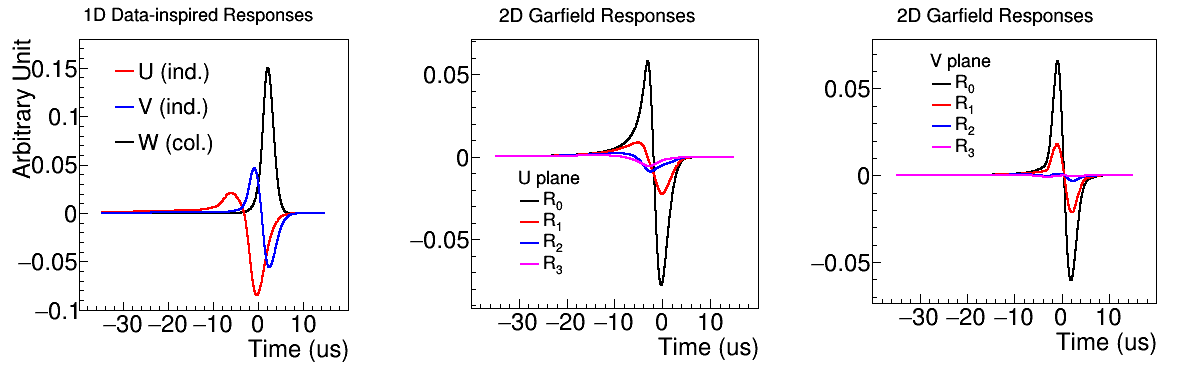
\includegraphics[width=\textwidth,clip,trim=15cm 0 15cm 0]{overall_response.png}      
      \scriptsize

      2D equivalent (from
      \href{http://www-microboone.fnal.gov/publications/publicnotes/MICROBOONE-NOTE-1017-PUB.pdf}{uB signal note})
    \end{column}
  \end{columns}
      \textbf{Preliminary, hot off the press!}

\end{frame}


\section{To Do}

\begin{frame}
  \frametitle{Next steps}

  \begin{itemize}
  \item More validation with 2D and Leon's 3D FEM work.
  \item Initial results \textbf{unfortunately} very similar to 2D!
    \begin{itemize}
    \item Just 2D$\to$3D not sufficient!?
    \item Go to +/- 10 neighbor wires for good 2D-deconvolution.
    \item Computation increases $\sim$ linearly with number of wires 
      \begin{itemize}
      \item[$\rightarrow$] (for BEM, FEM is $N^2$!).
      \end{itemize}
    \end{itemize}
  \item Implement \textbf{protoDUNE/SP and DUNE FD} geometries!
    \begin{itemize}
    \item Many more weighting fields needed due to non-uniform wire crossing pattern
    \item Need $\sim$30 unique $\vec{E}_{weight,k}$ instead of 3.
    \item Can look at ``edge effects'' such as at APA boundaries.
    \end{itemize}
  \end{itemize}


  \vfill

  \textbf{Anyone wanting to get involved is welcome!}
\end{frame}

\section{Software}


\begin{frame}[fragile]
  \frametitle{LARF - \textbf{L}iquid \textbf{Ar}gon TPC \textbf{F}ield Calculator}

  Some features:
  \begin{itemize}
  \item Handles pretty much everything with a simple \textbf{command line interface} and \textbf{configuration file}.
  \item Standard Python installation.
    \begin{itemize}
    \item Heavy lifting: \href{http://www.bempp.org/}{BEM++}, \href{http://gmsh.info/}{GMSH} and Numpy.
    \end{itemize}
  \item Results stored in Sqlite3 database with result provenance.
  \item Multiple, common data export methods (\texttt{.npz}, \texttt{.vtk})
    \begin{itemize}
    \item Playes well with \href{http://www.paraview.org}{paraview}!
    \end{itemize}
  \item[$\rightarrow$] \textbf{users/developers welcome}.
  \end{itemize}

  Code and docs on GitHub:
  \begin{center}
    \url{https://github.com/brettviren/larf}.    
  \end{center}

  \scriptsize Warning: docs need a refresh, contact me before reading so I can clean up.
\end{frame}

\section{}

\begin{frame}
  \begin{center}
      \Huge extras
  \end{center}
\end{frame}

\begin{frame}[fragile]
  \frametitle{Stepping}
  Evolution of position $\vec{r}_k \equiv \vec{r}(t_k)$ from step $k$ to $k+1$:
  \begin{center}
    $\vec{r}_k \rightarrow \vec{r}_{k+1} = \vec{r}_k + \vec{v}(\vec{r}_k) \times \Delta t_k$
  \end{center}
  Use \textbf{Adaptive Runge-Kutta + Cash/Karp} ($\sim 5^{th}$ order)
  \begin{itemize}
  \item From Numerical Recipes
  \item Take two different 6th order steps.
  \item Distance between each estimates error.
  \item Adjust $\Delta t_{k+1}$ based on error
  \item Hugely more efficient than simple RK4
  \item Must still watch for stepping to get stuck at maximum.
  \end{itemize}
\end{frame}

\begin{frame}[fragile]
  \frametitle{Induced Current (Krabby) Field for U Wire}
  \begin{columns}
    \begin{column}{0.8\textwidth}
      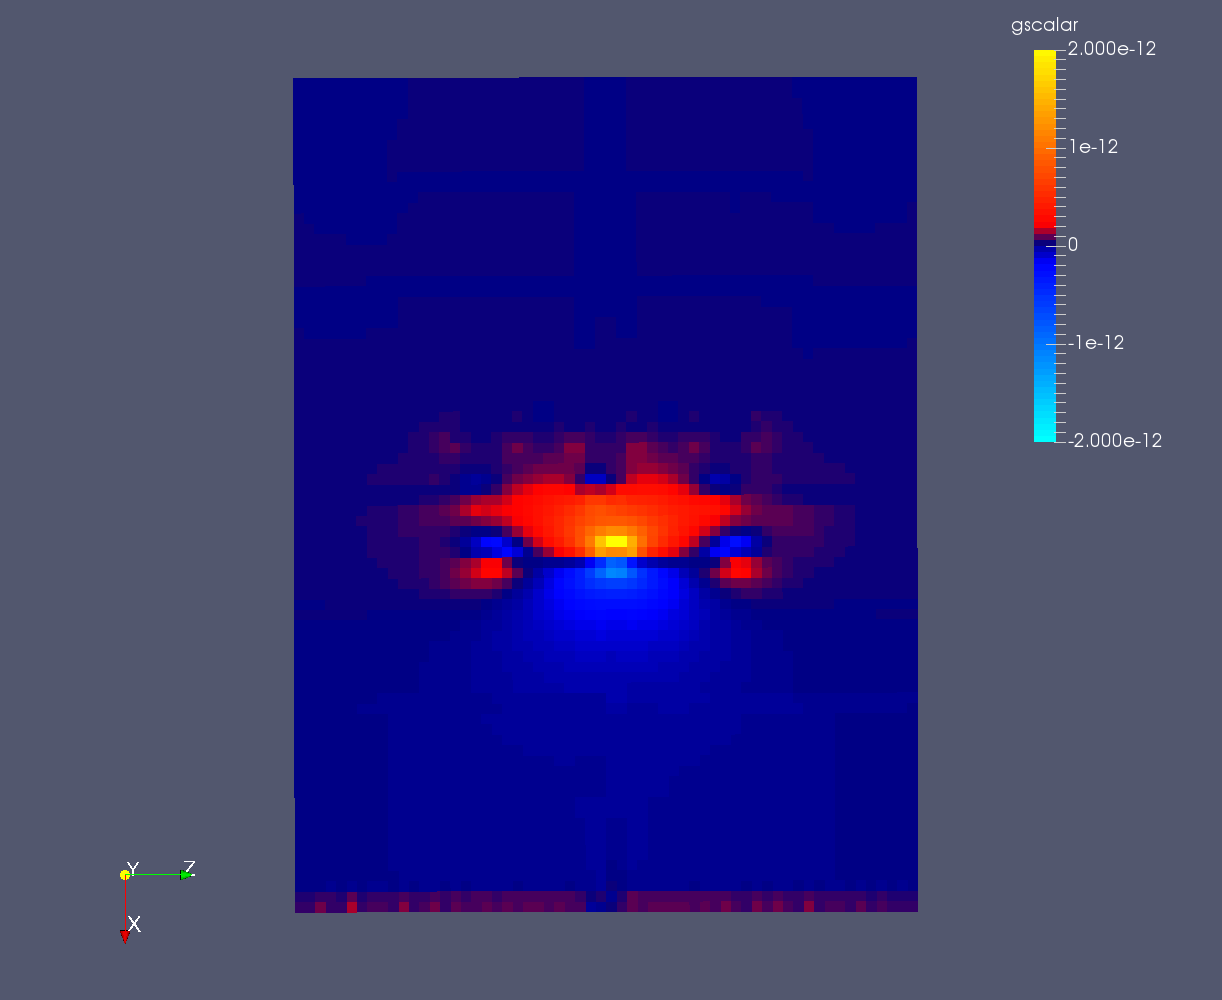
\includegraphics[width=0.9\textwidth]{demon-current.png}      
    \end{column}
    \begin{column}{0.2\textwidth}
      \includegraphics[height=2cm]{098Krabby.png}          
    \end{column}
  \end{columns}

  \begin{center}
  \footnotesize
  U-wire at center, drift goes upward, Y-Z slice, 0.5 mm voxels, current in Amps.
    
  \end{center}
\end{frame}


\end{document}